\chapter{Функционалности} \label{UseCases}
\emph{Ма колико изгледало наивно и просто направити дизајн који ће привући корисника, док не кренете да правите апликацију, не схватите колико немате појма шта просечан корисник хоће. Стога након пажљивог разматрања направљено је пет "екрана" из којих кориснк приступа одговарајућим функционалностима које ће бити изложене у даљем тексту}

\section{Почетни екран}

\subsection{Основни}
\begin{figure}[htb!]
\begin{center}
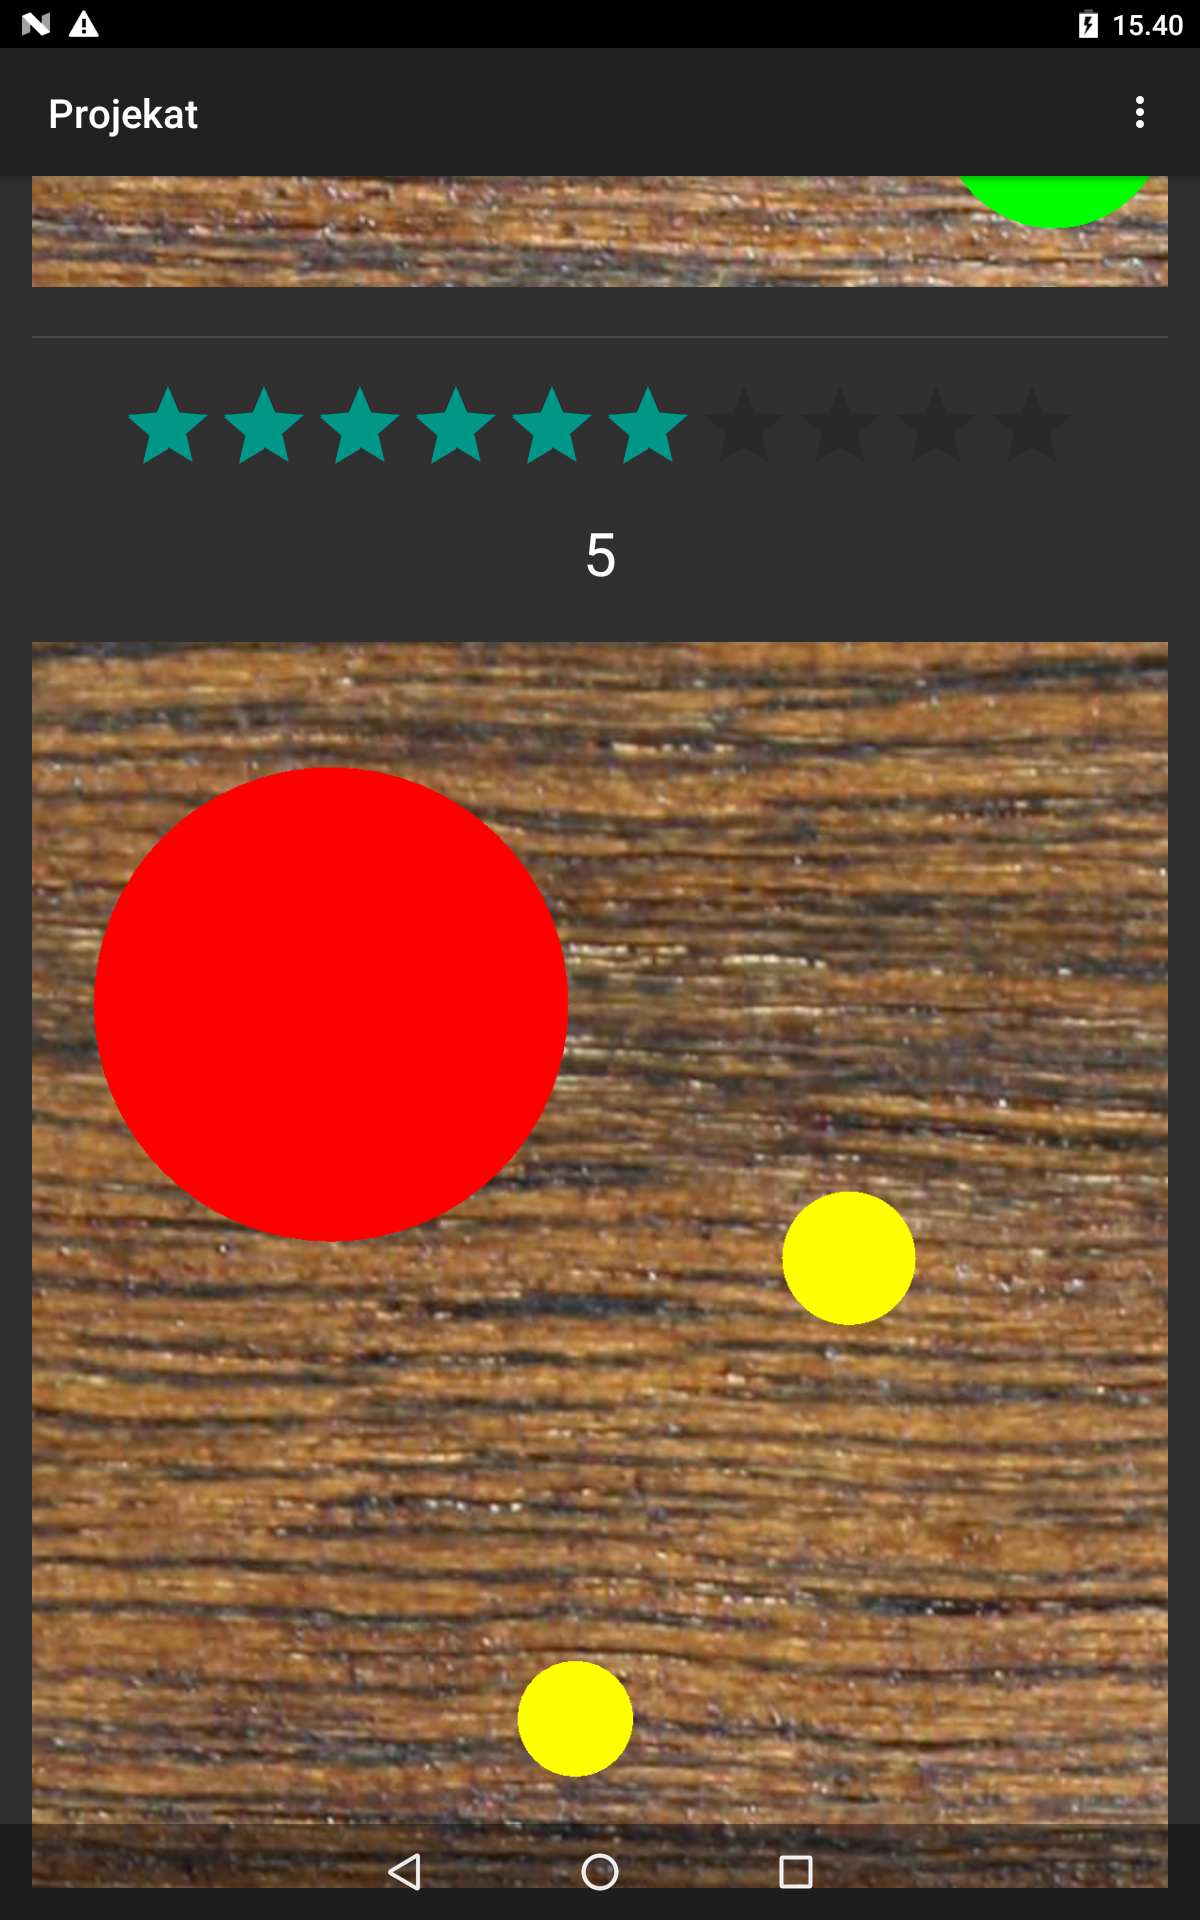
\includegraphics[scale=.1]{pictures/main/Basic}
\caption{Почетни екран}\label{fig:mainBasic}
\end{center}
\end{figure}
Кад корисник покрене апликацију појављује му се листа полигона које може да игра, са изгледом полигона (слика \ref{fig:mainBasic}). Такође изнад изгледа полигона налазе се његово име и тежина. Ово омогућава да кориснику почетнику одабере ниво прикладан за њега, или експерту да се окуша са нечим тежим. Изглед полигона је скалиран да одговара оном који ће бити у игрици. Кликом на било који од полигона у листи покреће му се игра за тај полигон.

\subsection{Meни}
\begin{figure}[htb!]
\begin{center}
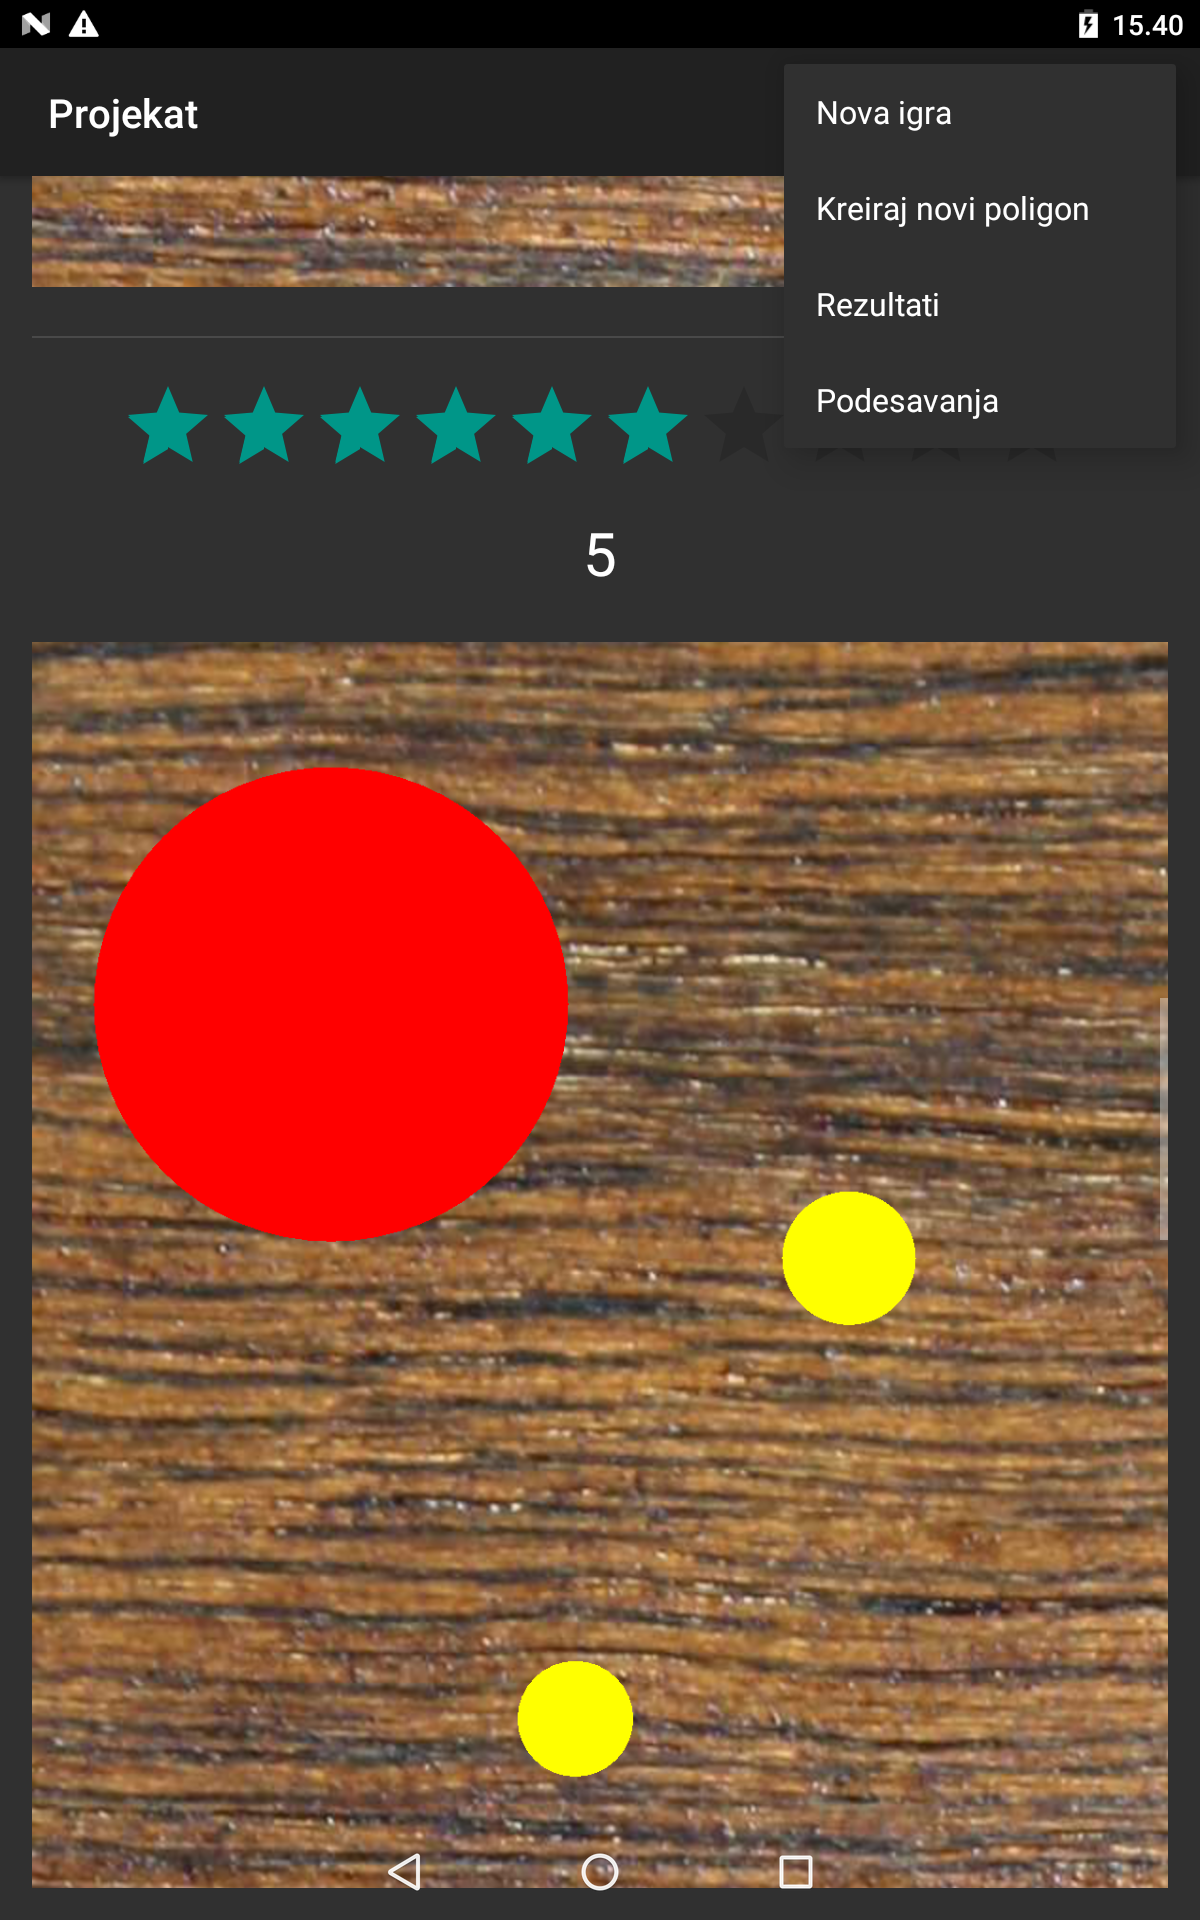
\includegraphics[scale=.1]{pictures/main/Menu}
\caption{Мени}\label{fig:mainMenu}
\end{center}
\end{figure}
Корисник све време на врху прозора има мени који отвара ако прстом кликне на три тачке. Из менија који се појави (слика \ref{fig:mainMenu}) корисник може да одабере једну од 4 опције. Прва опција започиње нову игру, али у режиму од више нивоа који су насумично генерисани. Друга опција отвара нови екран у ком корисник прави свој полигон. Трећа опција отвара нови екран резултати, где корисник може да види све резултате претходних игри, као и других играча. Четврта опција отвара подешавања за игру, која корисник може да мења.


\subsection{Опције полигона}
\begin{figure}[htb!]
\begin{center}
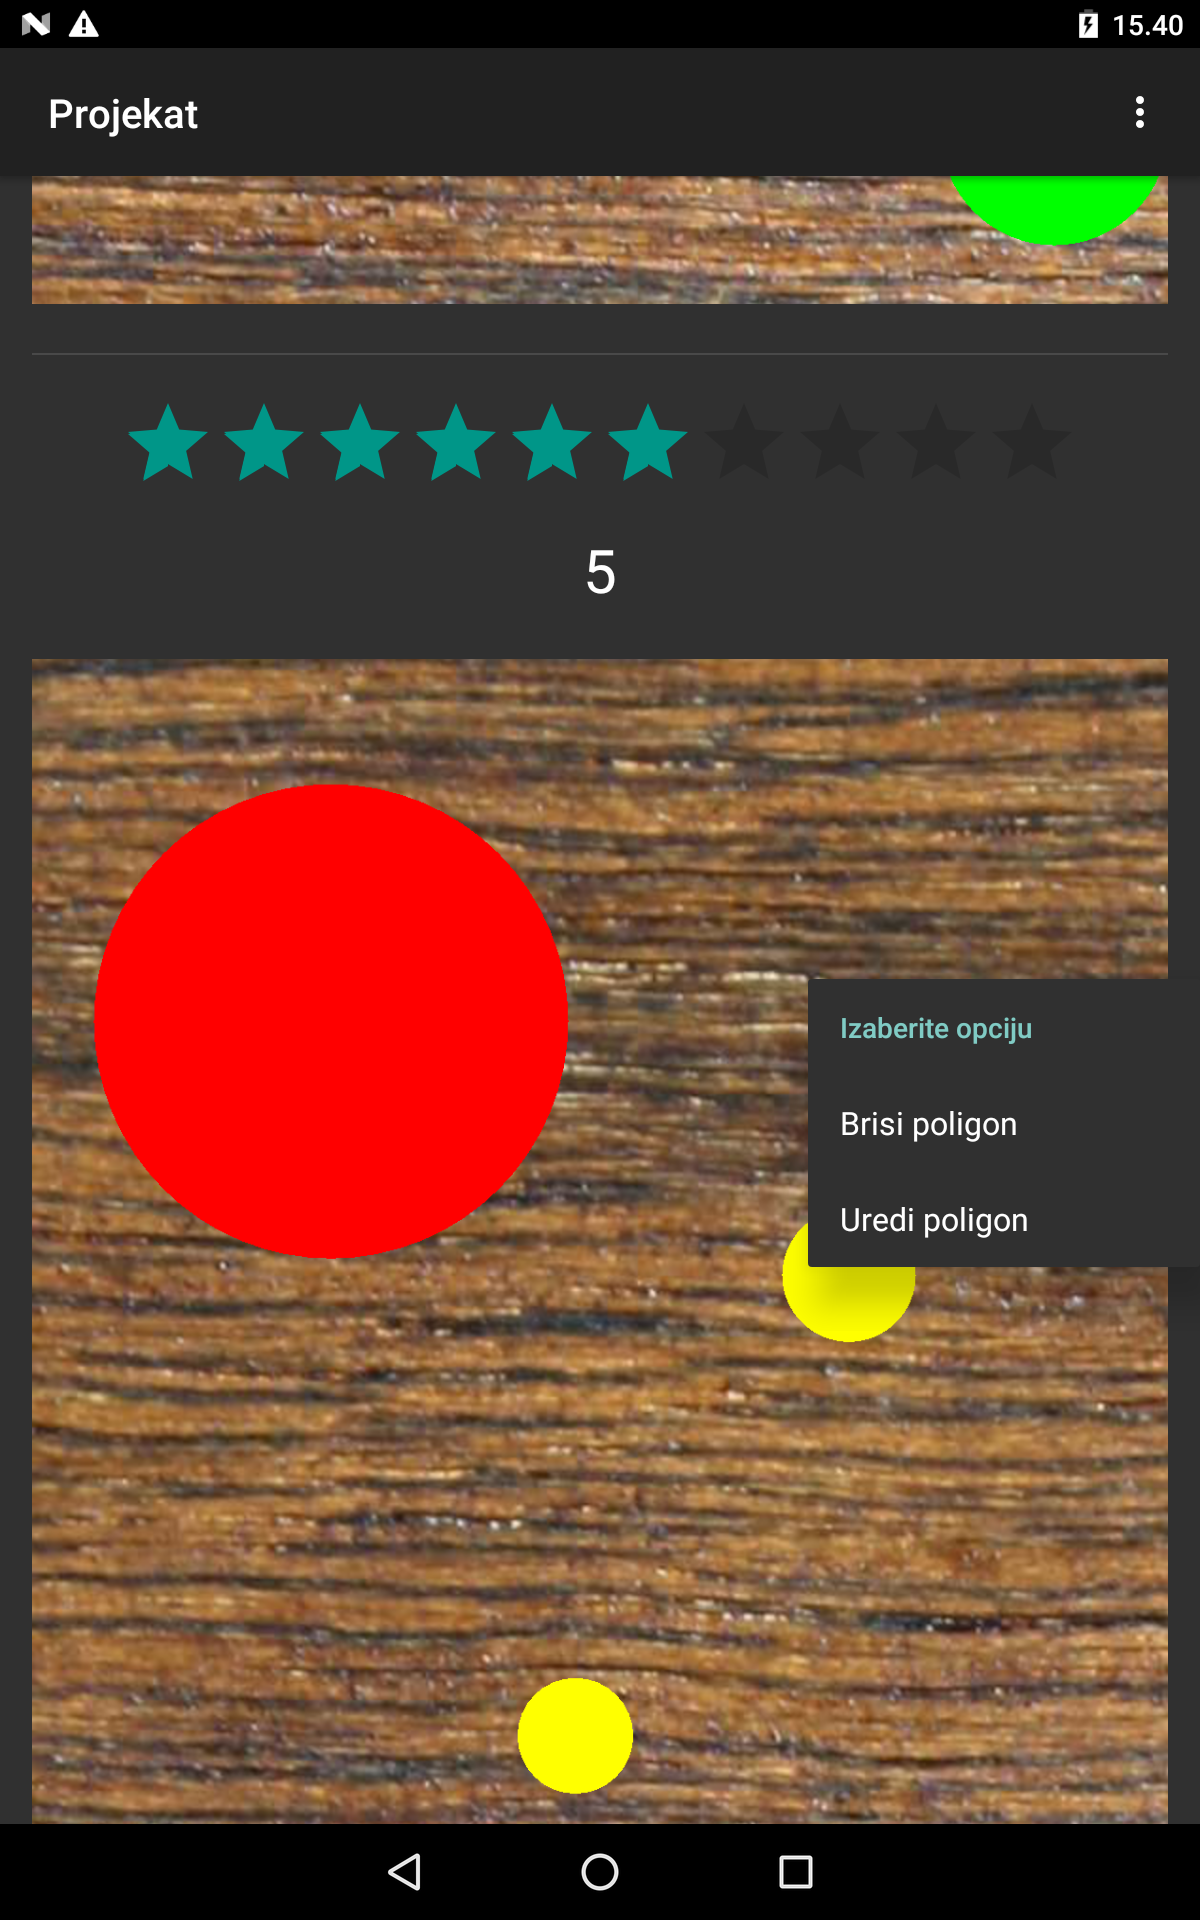
\includegraphics[scale=.1]{pictures/main/PolygonMenu}
\caption{Падајући мени везан за полигон}\label{fig:mainPolygonMenu}
\end{center}
\end{figure}
Корисник задржавањем прста на полигон добија падајући мени (слика \ref{fig:mainPolygonMenu}) са две опције. Прва опција брише полигон из целе игре. А друга омогућава његово уређивање, тако што отвара нови прозор са датим полигоном.

\section{Игра}\label{game}
\begin{figure}[htb!]
\begin{center}
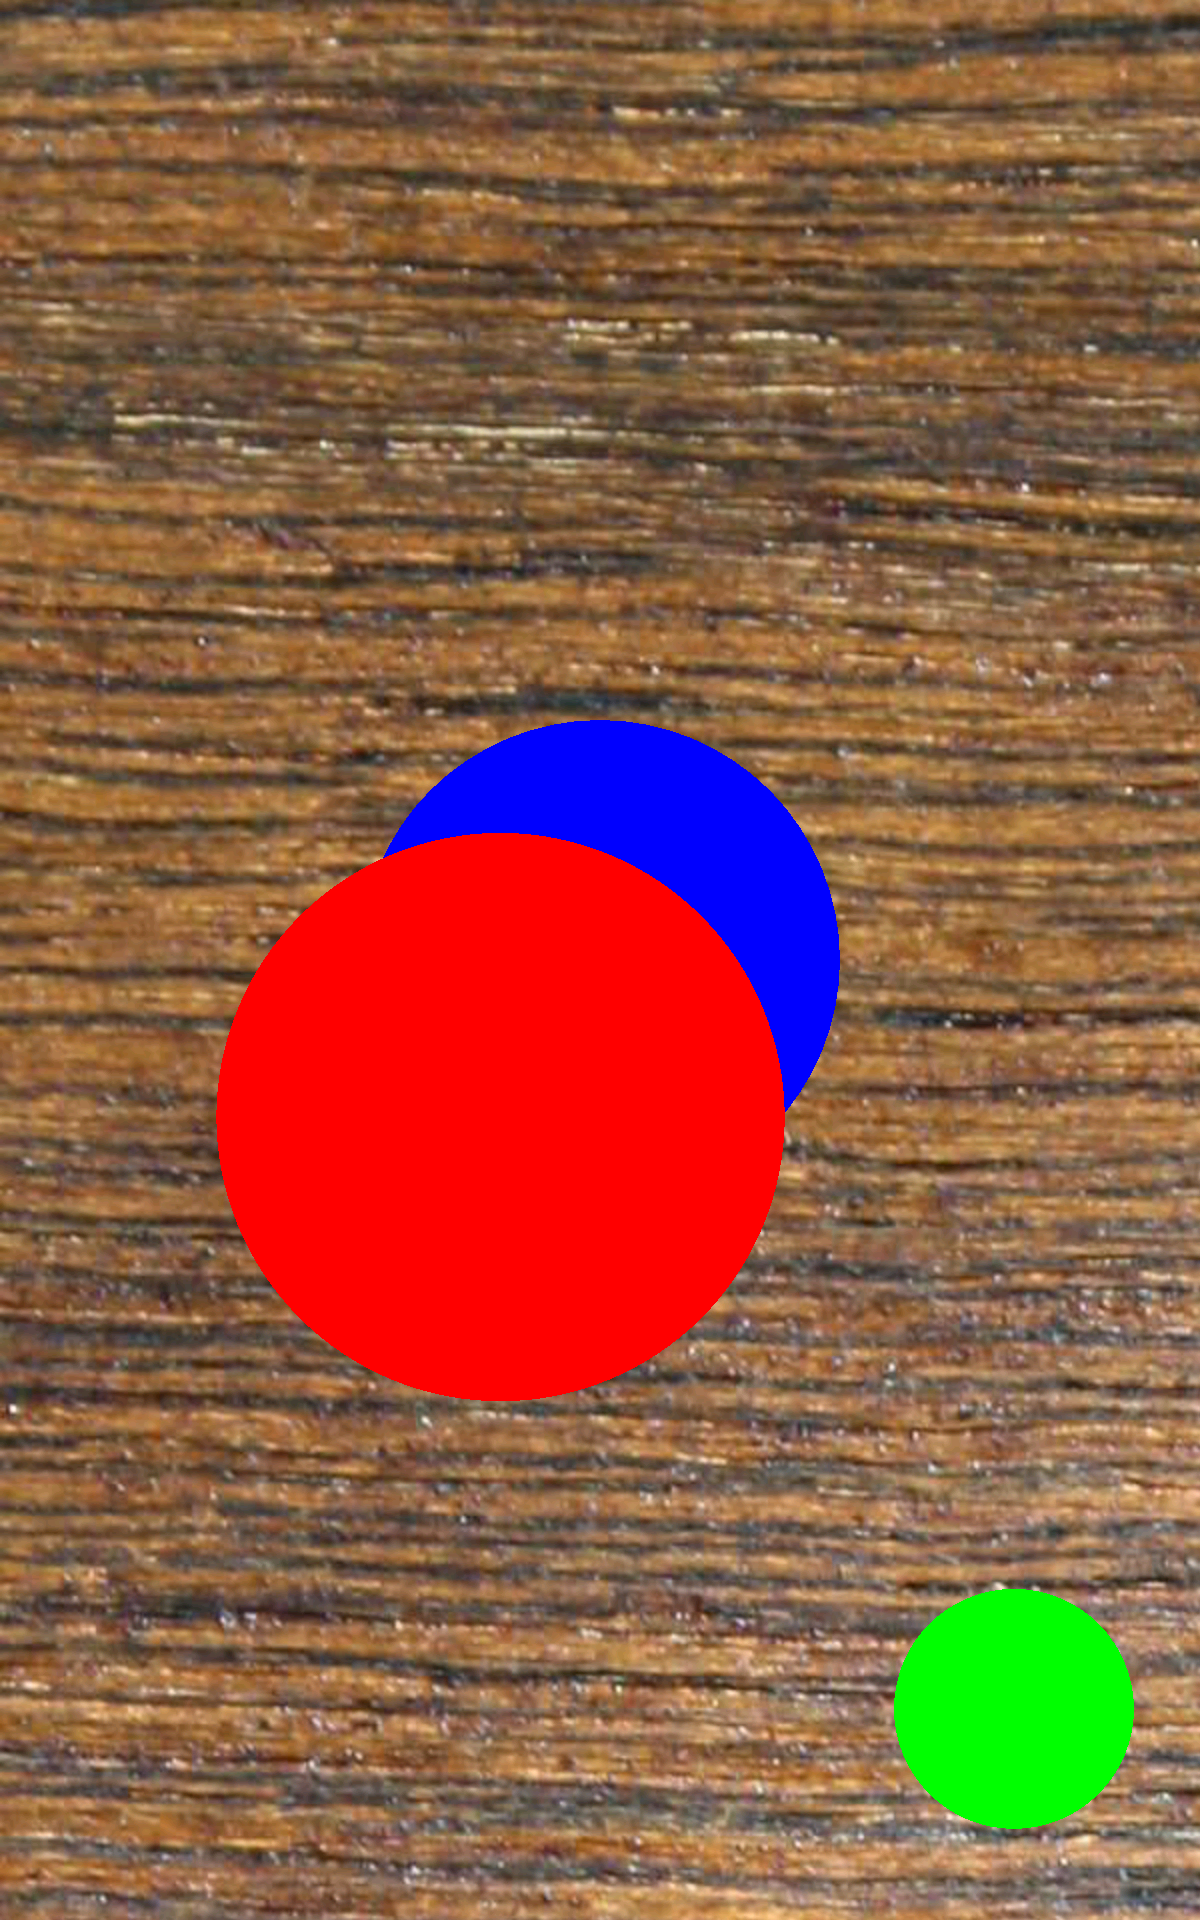
\includegraphics[scale=.1]{pictures/game/game}
\caption{Тренутак у игри}\label{fig:gameGame}
\end{center}
\end{figure}


Постоје два мода играња. Први мод је обичан у ком је циљ да црвену лопту корисник убаци у зелену рупу за што краће време (слика \ref{fig:gameGame}). Што му је време краће, биће боље рангиран на листи за тај полигон. Други мод је авантуристчки који омогућава кориснику да игра десет насумичних нивоа заредом који су поређани по растућој тежини и биће рангиран на посебној листи  за тај мод. Корисник има неколико типова препрека на које може да наиђе (слика \ref{fig:createPolygonBasic}). Типови препрека:
\begin{enumerate}
	\item Зид (ивица екрана и жути правоугаоник) - лопта се одбија од зида под истим углом којим улази. Губитак енергије током судара зависи од коефицијента подешеног у подешавањима.
	\item Стуб (жути круг) - исто као зид, са тим да је кружног облика.
	\item Амбис (црни круг) - лопта кад упадне у њега играч губи игру.
	\item Вртлог (плави круг) - покушава да увуче лопту у њега, и потом у зависности од брзине баца из њега или га врти.
	\item Крај (зелени круг) - кад лопта упадне у њега корисник је победио дати полигон.\footnote{Амбис, вртлог и крај кад лопта их дотакне вуку је ка себи одређеном силом}
\end{enumerate}
Лопта све време добија брзину у зависности од силе која делује на Android уређаја. На лопту у сваком тренутку делује трење од стране подлоге које покушава да је врати у стање мировања. У сваком тренутку корисник може да изађе из одговарајућег полигона, али неће му бити сачувано ништа што је играо.
\subsection{Игра побеђена}
\begin{figure}[htb!]
\begin{center}
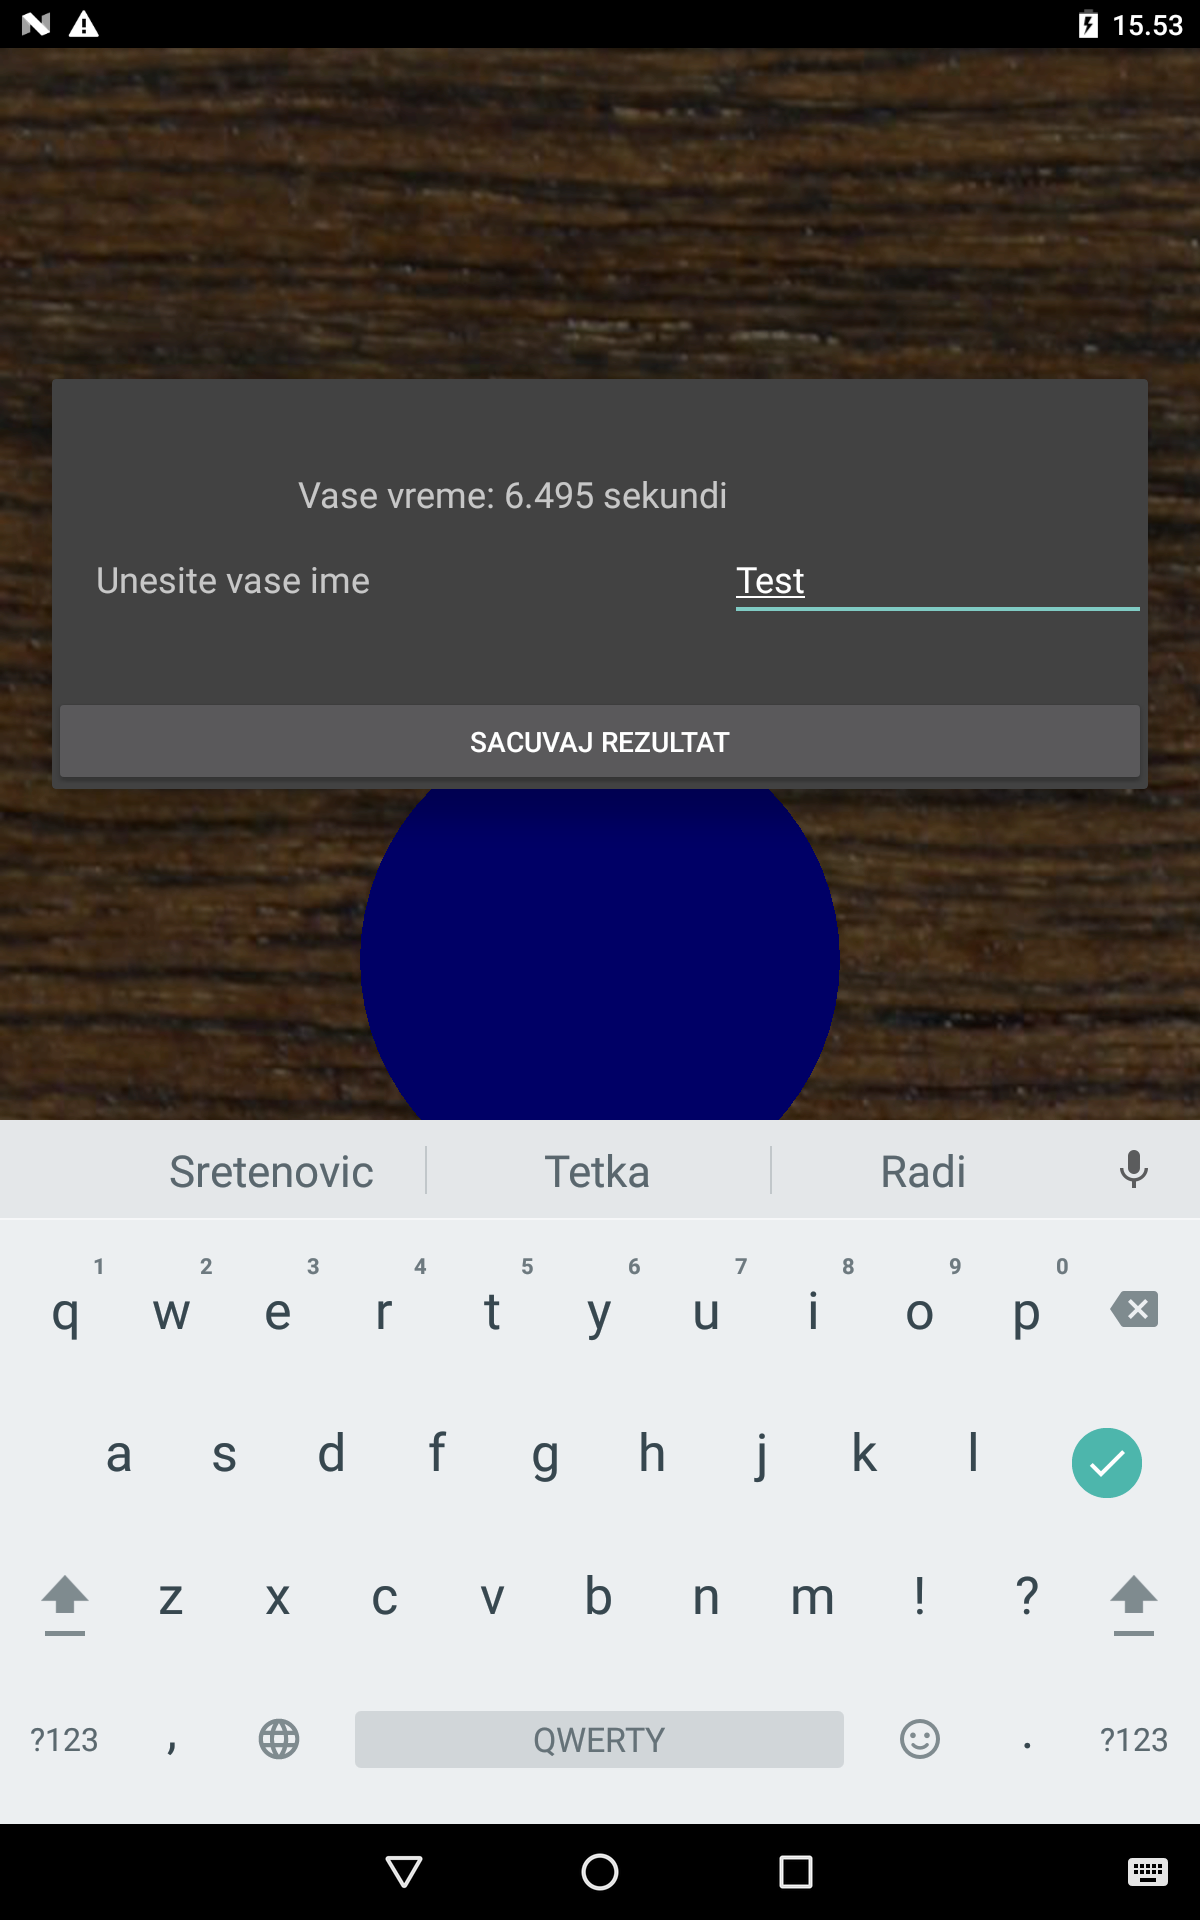
\includegraphics[scale=.1]{pictures/game/gameWon}
\caption{Дијалог кад победи}\label{fig:gameGameWon}
\end{center}
\end{figure}


\begin{figure}[htb!]
\begin{center}
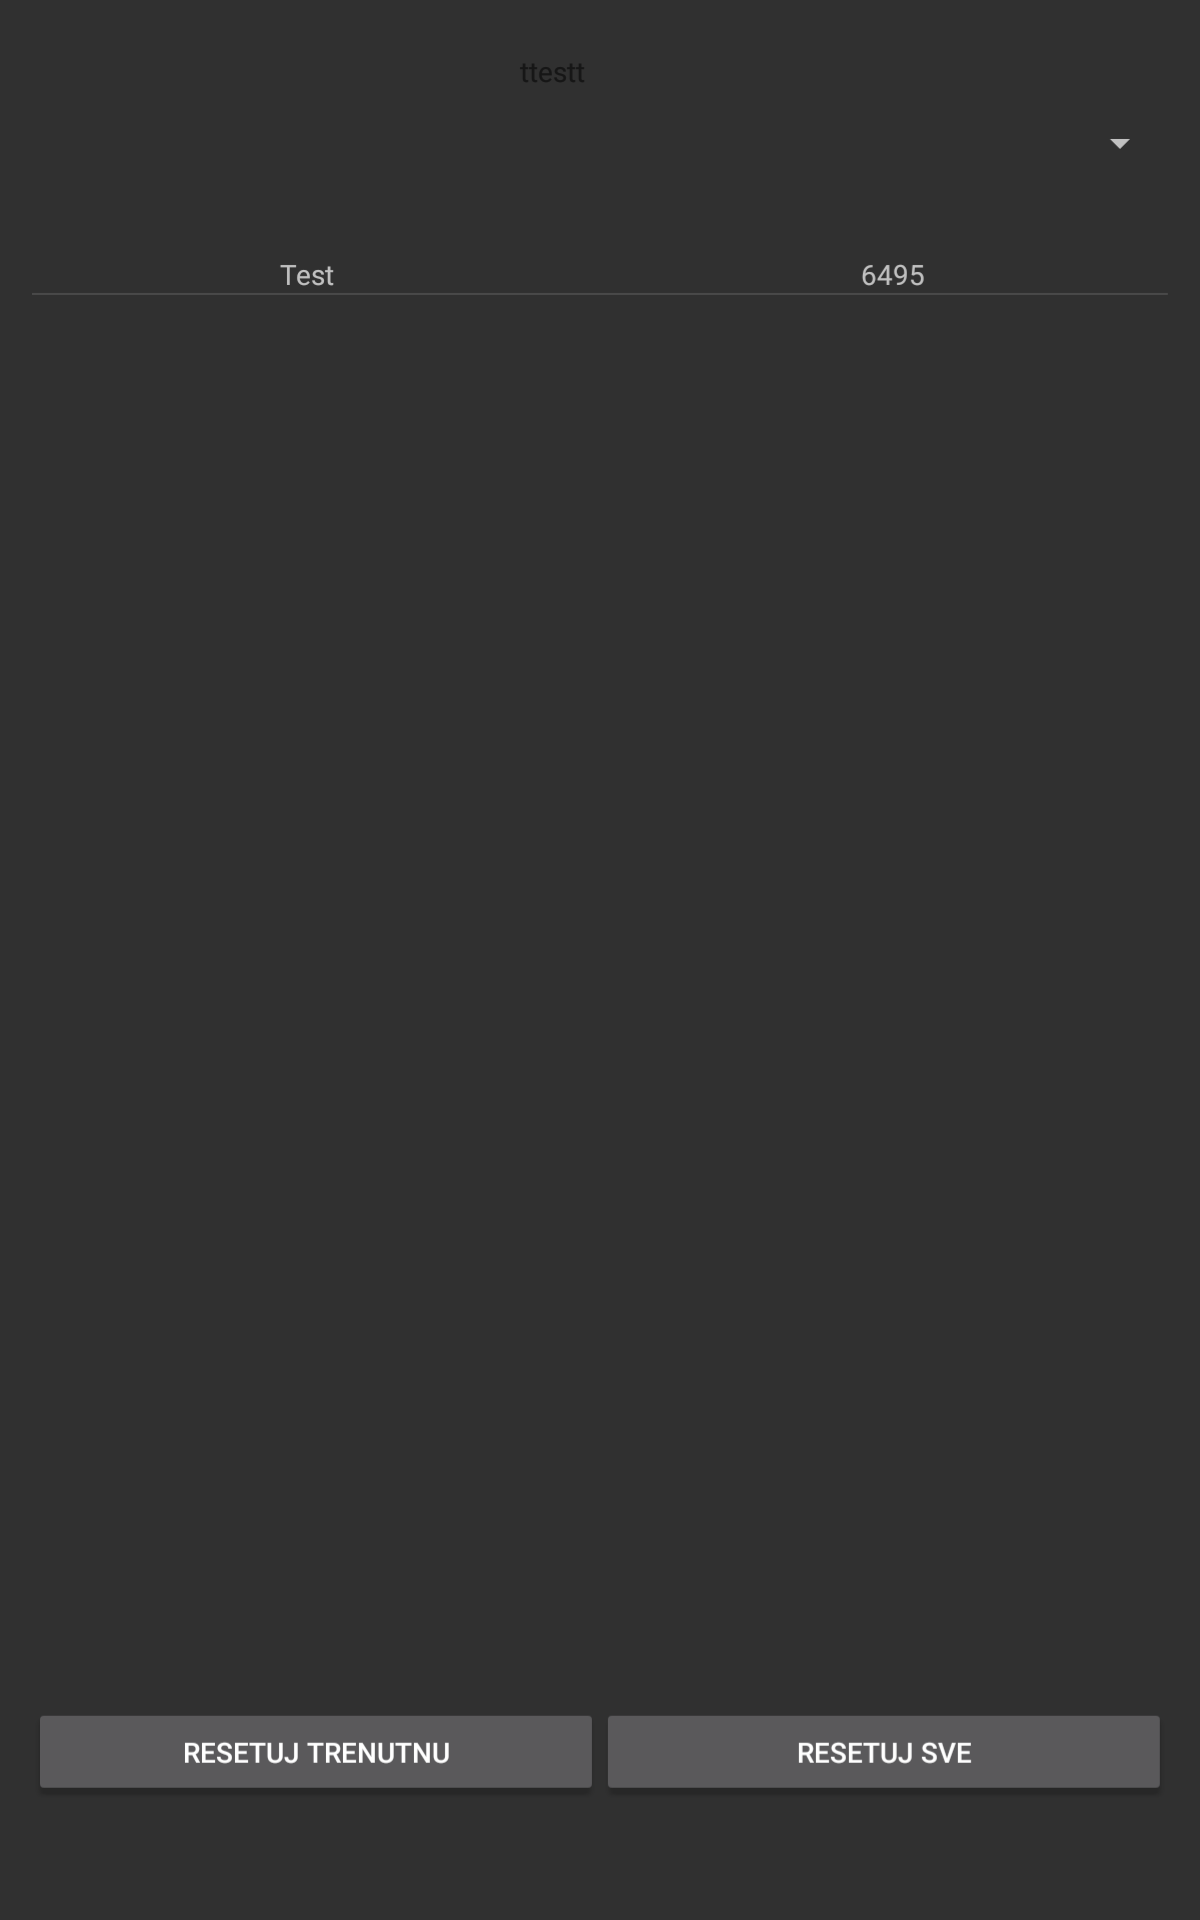
\includegraphics[scale=.1]{pictures/game/gameHighScore}
\caption{Листа резултата за полигон који је победио}\label{fig:gameGameHighScore}
\end{center}
\end{figure}

Кад корисник убаци лопту у зелену рупу, искаче му дијалог (слика \ref{fig:gameGameWon}). На дијалогу пише време, као и нуди кориснику да унесе своје име. Кад кликне на дугме \emph{SACUVAJ REZULTAT} корисников резултат се чува у листи резултата за тај плигон и отвара листа резултата за исти(слика \ref{fig:gameGameHighScore}).
\subsection{Игра изгубљена}
\begin{figure}[htb!]
\begin{center}
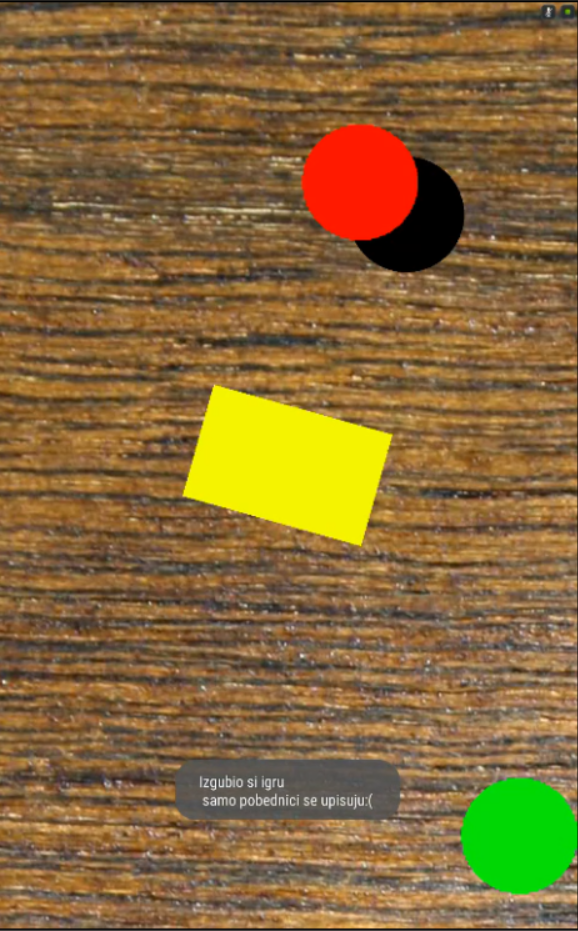
\includegraphics[scale=.4]{pictures/game/gameLose}
\caption{Обавештење кад корисник изгуби}\label{fig:gameLose}
\end{center}
\end{figure}
Када корисник упадне у амбис изађе му обавештење да је изгубио игру (слика \ref{fig:gameLose}). 

\section{Прављење полигона}
Постоје два мода у која корисник може да уђе кад уређује полигон. 
\\ \indent Један је мод уређивања, у ком се налази тако што или је кликнуо \emph{Uredi poligon} на почетном екрану или је сачувао полигон под неким именом. У овом моду кад корисник кликне назад аутоматски ће се чувати поруке и бити избацивана упозорења ако нешто није како треба (фали крајња позиција, почетна...). 
\\ \indent Други мод је обични мод и то је док корисник није сачувао полигон. У овом моду кад се кликне дугме назад, ништа неће бити сачувано. 
\subsection{Опције за уређивање полигона}
\begin{figure}[htb!]
\begin{center}
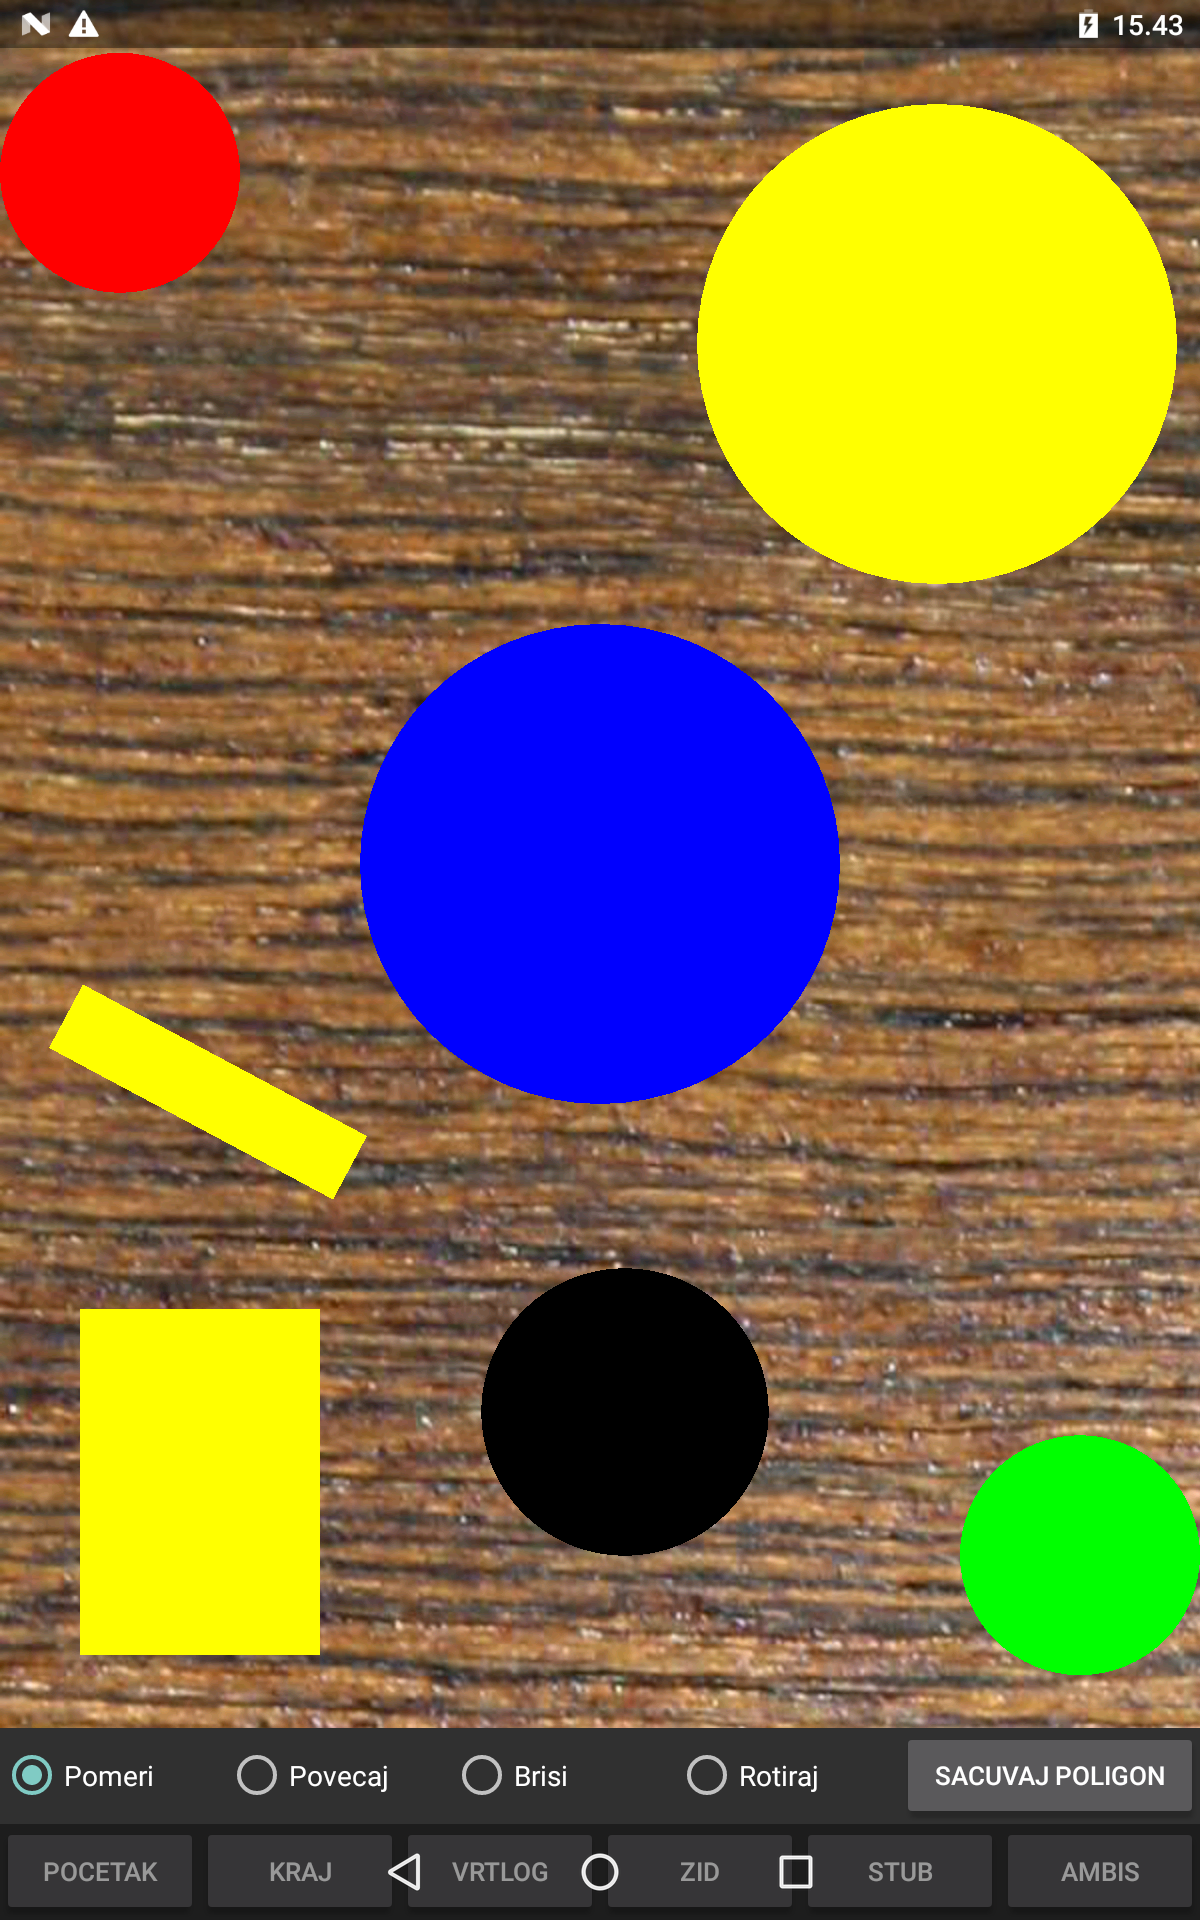
\includegraphics[scale=.1]{pictures/createPolygon/Basic}
\caption{Екран који корисник види кад уређује полигон}\label{fig:createPolygonBasic}
\end{center}
\end{figure}
Корисник има опције генерисања препрека за лопту наведеним у секцији \ref{game} кликтањем одговарајућег дугмета са именом. Такође може и да генерише почетну позицију лопте.  Поред тога са свим фигурама корисник може да ради једну од четири опције:
\begin{enumerate}
\item  \emph{Pomeri} - Помера одговарајућу фигуру на полигону тако да корисник мора да задржава прст на фигуи док је помера, Кад пусти, ту ће фигура бити померена. 
\item  \emph{Povecaj}- Повећава одговарајућу фигуру, тако да ако корисник одабере фигуру и помера прст, фигура ће се повећавати у односу на то где је његов прст (за круг ће крајња позиција прста означавати позицију тачке са кружнице, за правоугаоник позицију одговарајућег темена).
\item  \emph{Brisi} - Брише  одабрану фигуру са полигона.
\item  \emph{Rotiraj} - Ротира правоугаоник према позицији прста тако да одабрана права која је одређена центром правоугаоника и прстом ротира око центра пратећи прст, са том правом ротира и цео правоугаоник. 
\end{enumerate}

\subsection{Чување полигона}
\begin{figure}[htb!]
\begin{center}
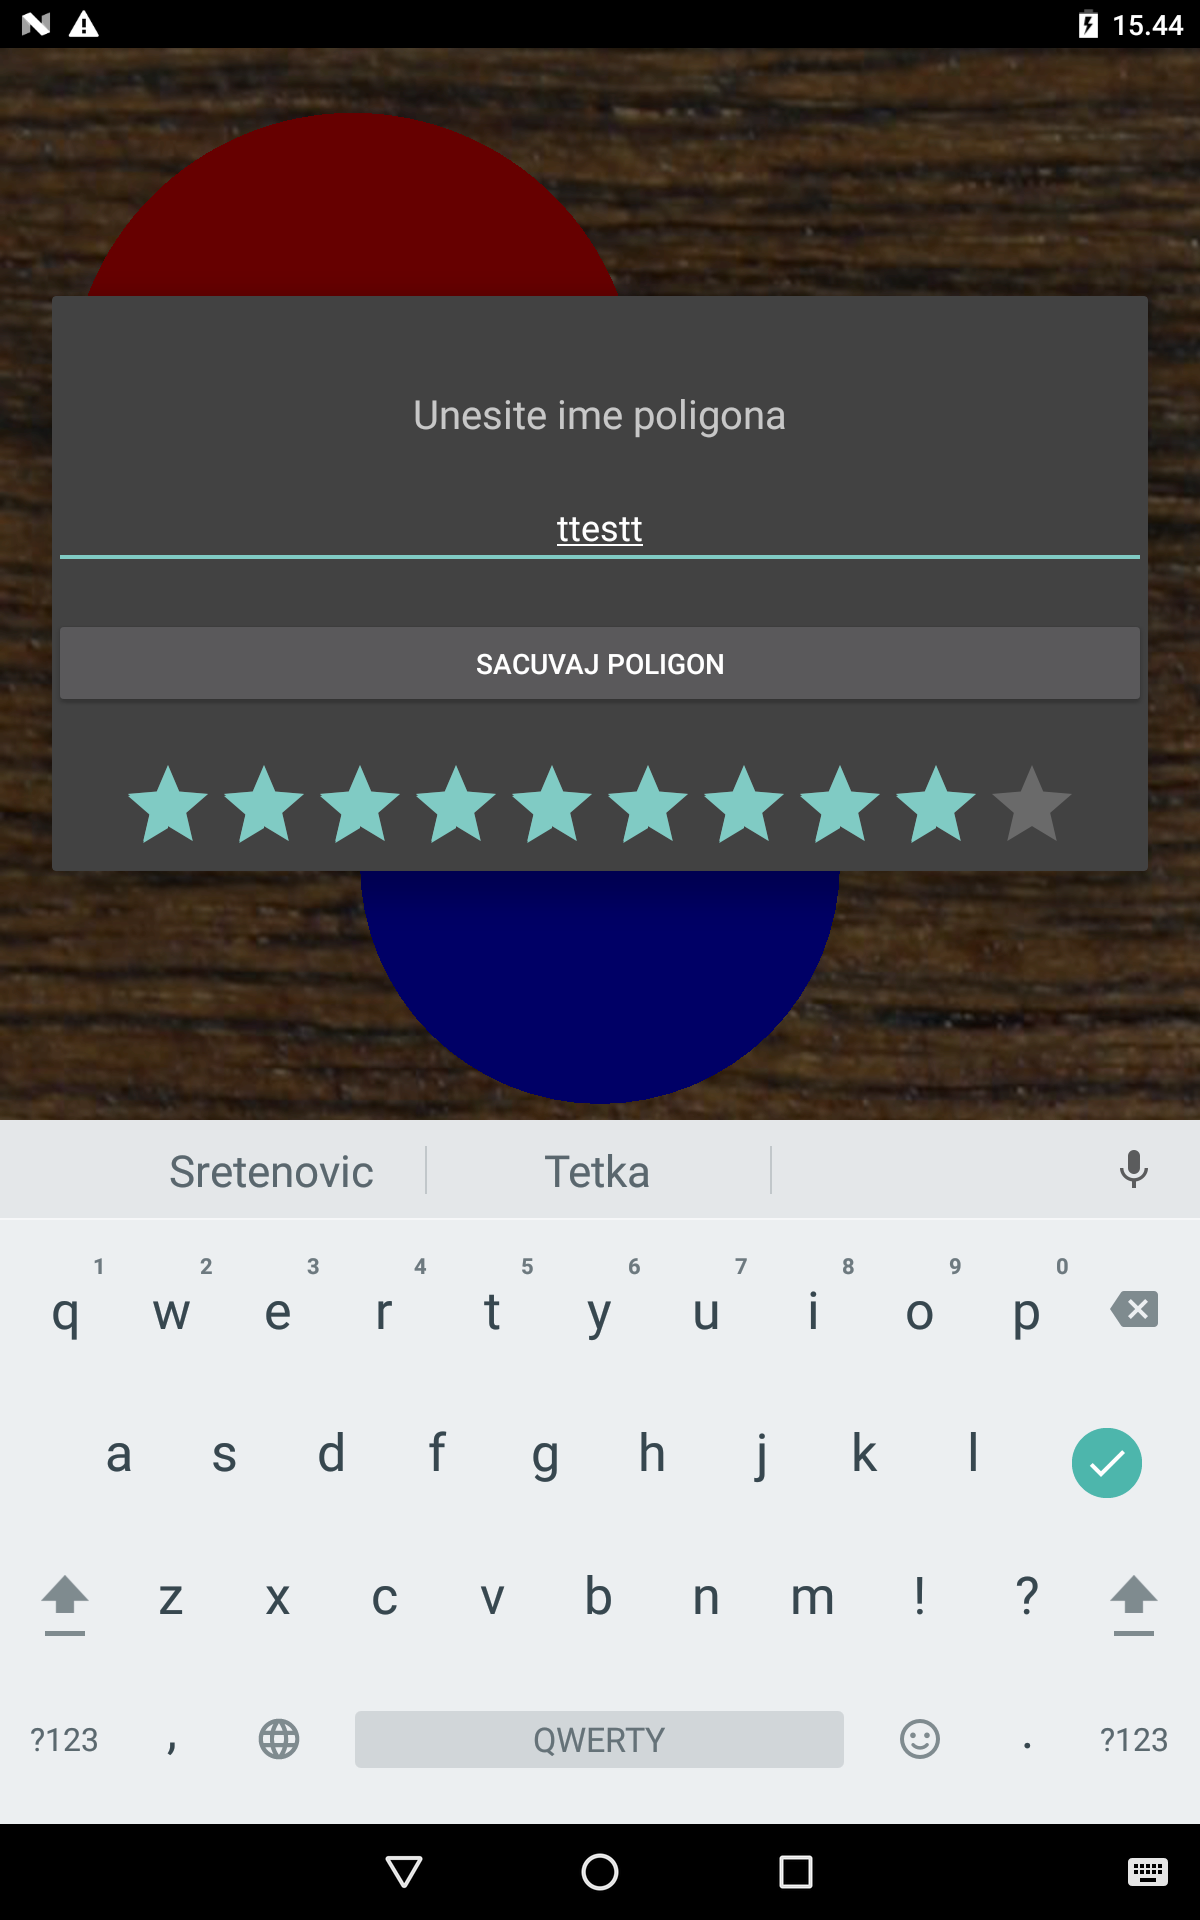
\includegraphics[scale=.1]{pictures/createPolygon/Save}
\caption{Дијалог који се појави кад корисник хоће да сачува полигон}\label{fig:createPolygonSave}
\end{center}
\end{figure}
На крају корисник кад заврши генерисање правоугаоника има дугме \emph{SACUVAJ POLIGON}. Тад се кориснику појављује дијалог на коме уноси тежину полигона као и име тог полигона. Кад кликне \emph{SACUVAJ POLIGON} на новом дијалогу, сачуваће полигон. Ако је постојао стари пребрисаће га.


\section{Резултати}
\begin{figure}[htb!]
\begin{center}
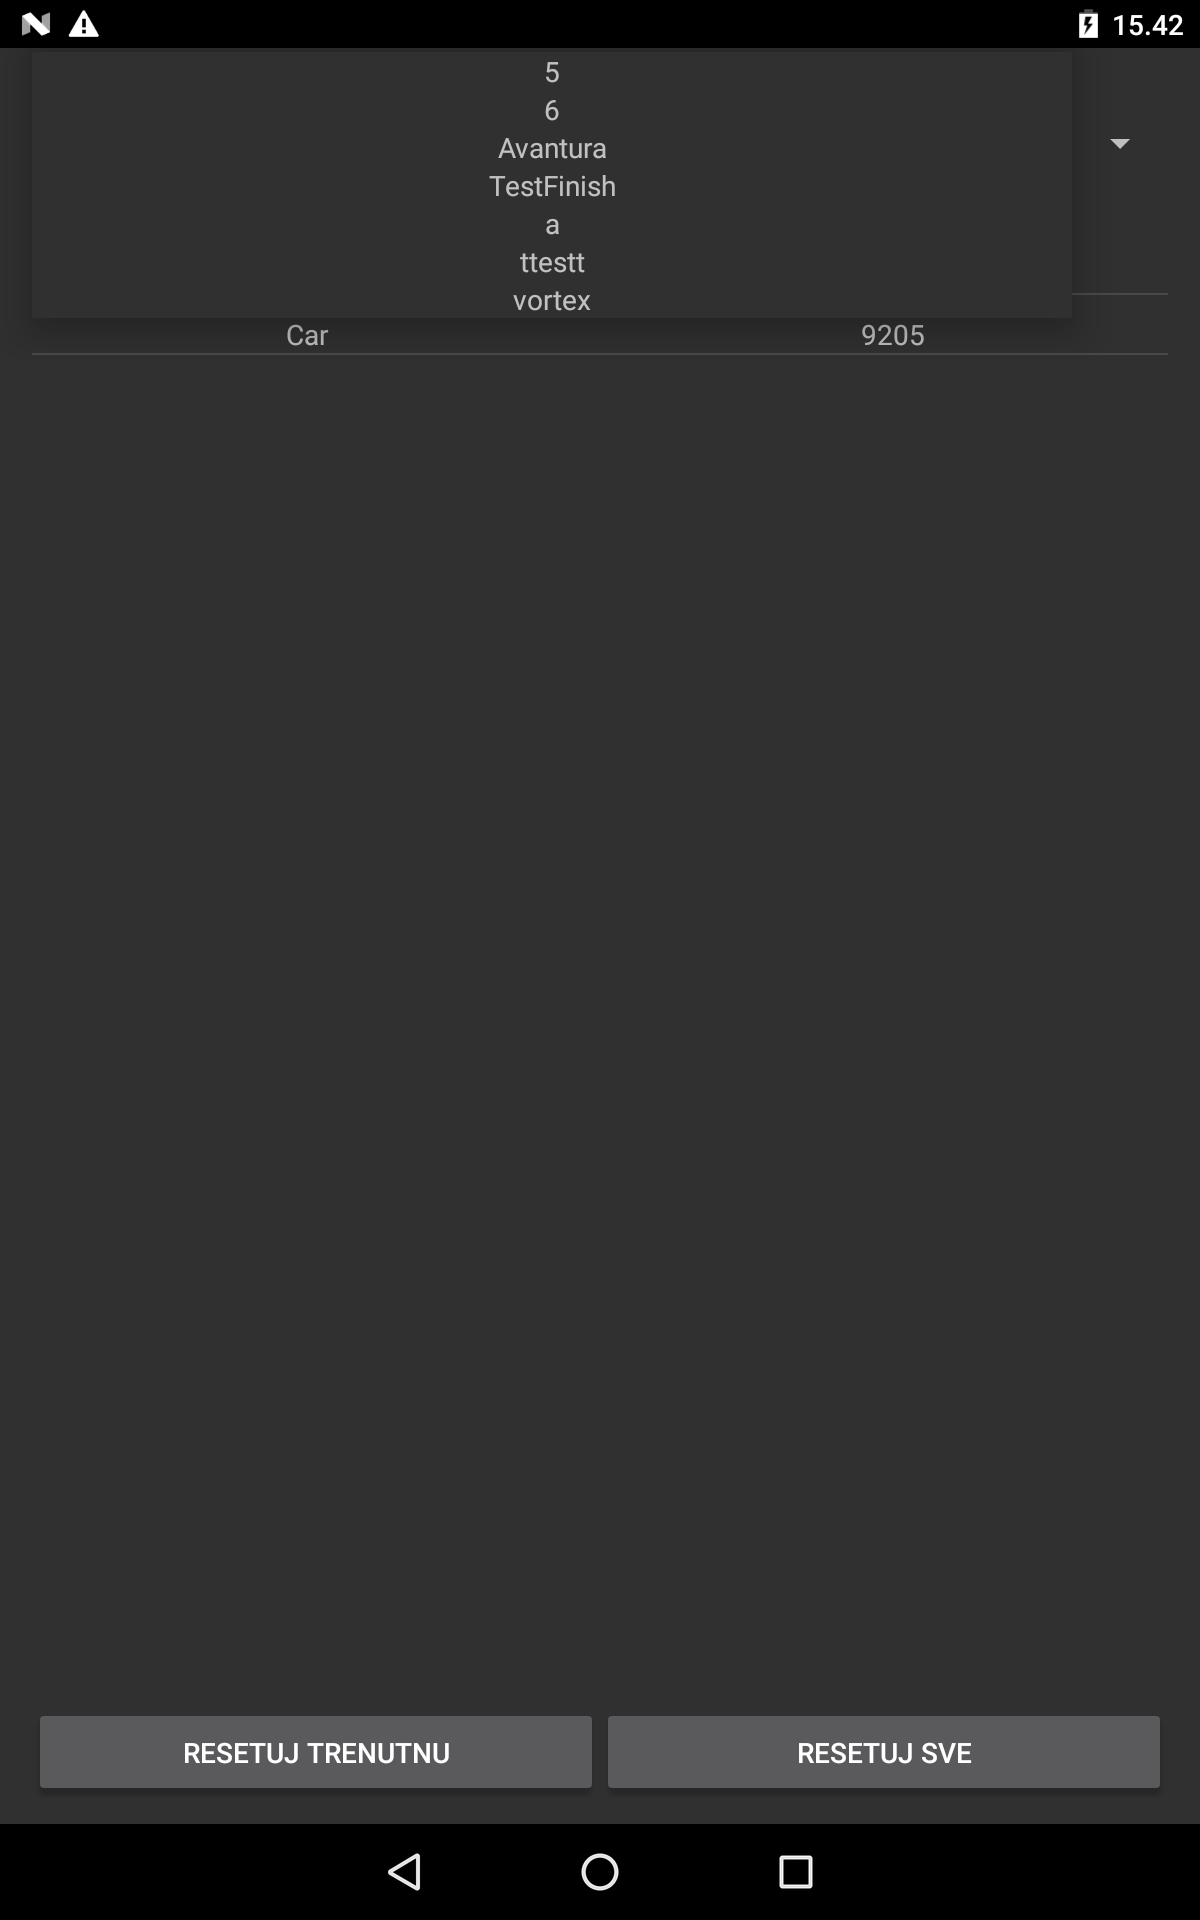
\includegraphics[scale=.1]{pictures/statistics/Choose}
\caption{Избор полигона за који хоће да се виде резултати}\label{fig:statisticChoose}
\end{center}
\end{figure}

\begin{figure}[htb!]
\begin{center}
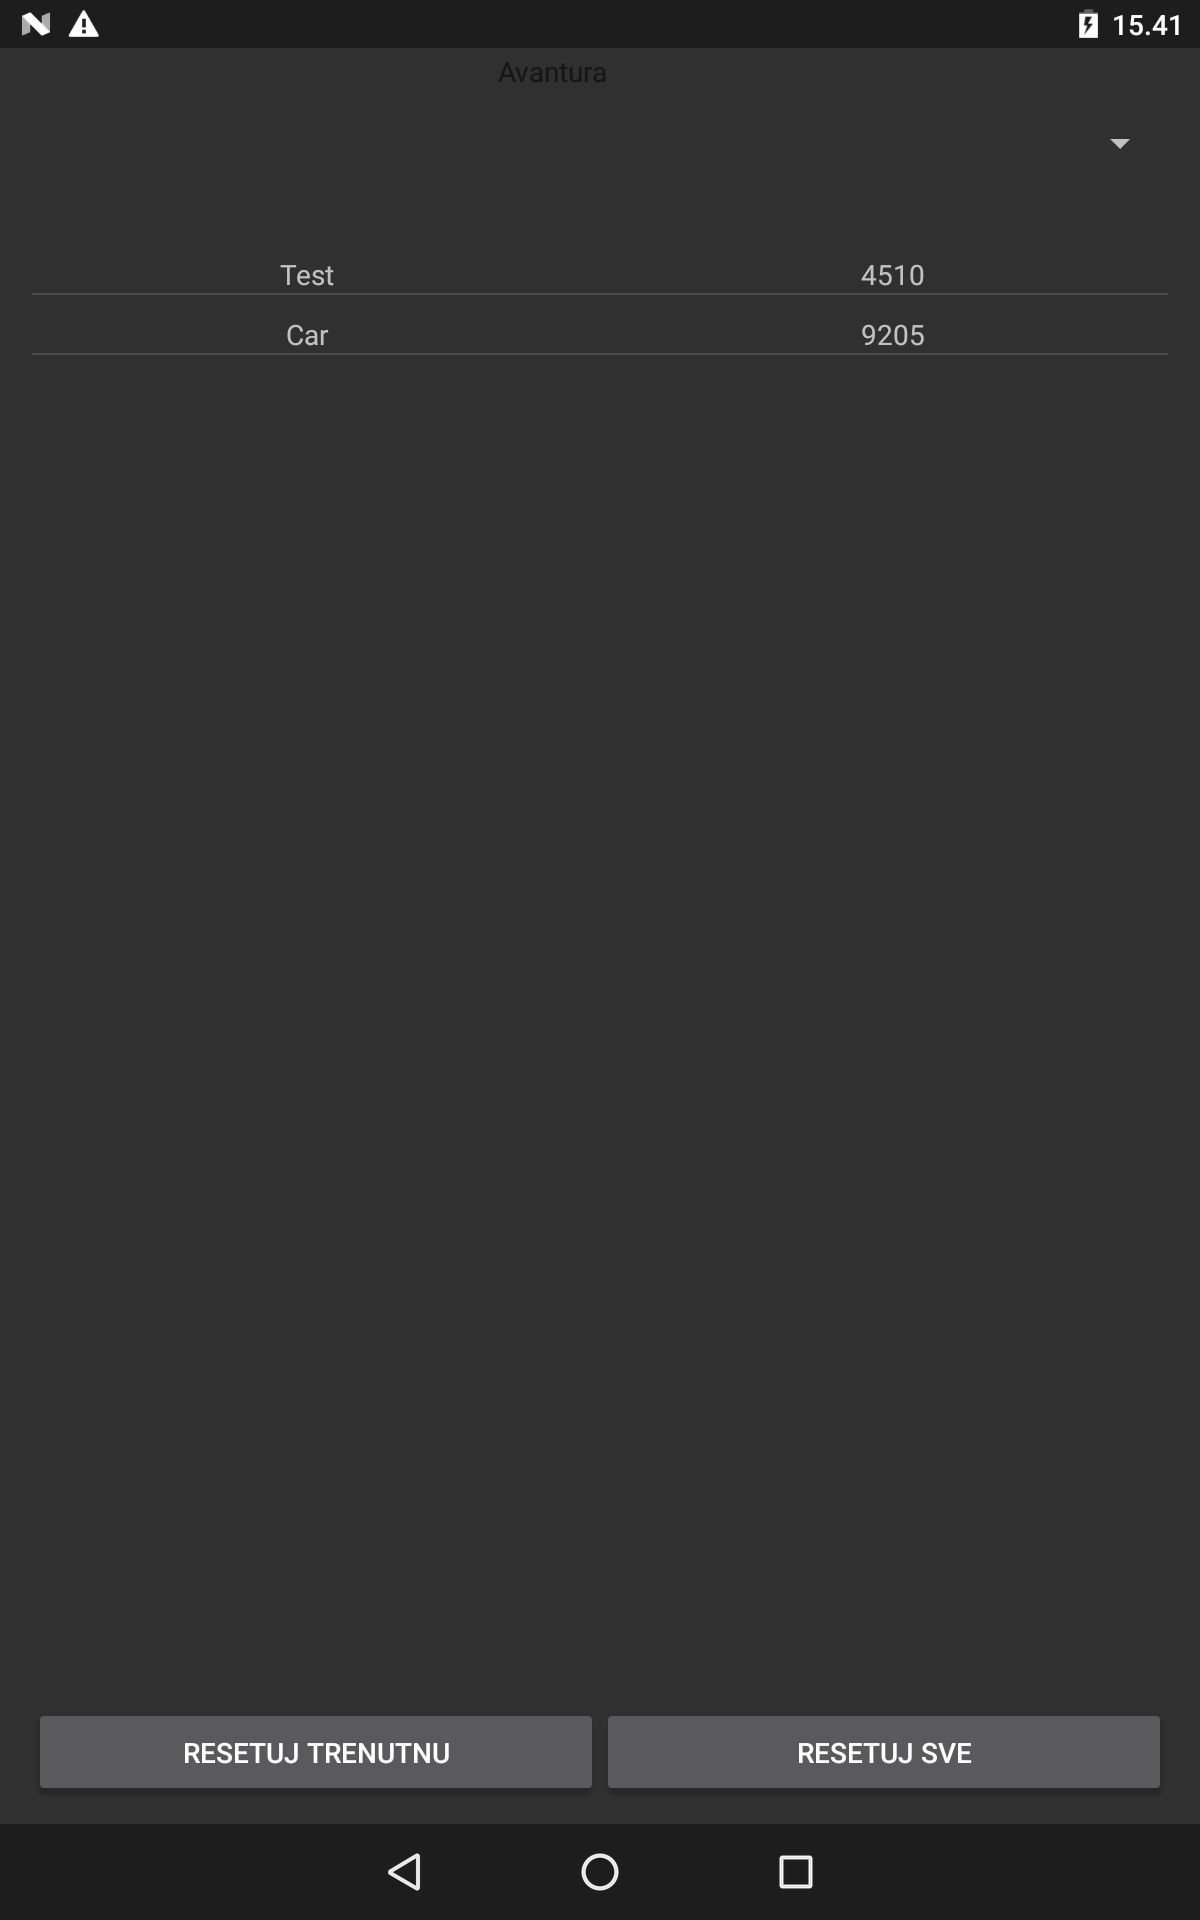
\includegraphics[scale=.1]{pictures/statistics/HighScore}
\caption{Листа резултата за одговарајући полигон}\label{fig:statisticHighScore}
\end{center}
\end{figure}
Корисник има опцију да види статистику за све полигоне које је играо, и који постоје . Такође има моућност да види и за авантура мод (под именом \emph{Avantura}). Корисник кликом на спинер бира одговарајући ниво за који хоће да прикаже резултате (слика \ref{fig:statisticChoose}) и потом, му се приказују резултати сортирани од најбољег ка најлошијем (\ref{fig:statisticHighScore}) у погледу времена. Корисник има могућност ресетовања листе резултата за један изабрани полигон притискањем дугмета \emph{RESETUJ TRENUTNU} или ресетовањем резултата свих листи са притискањем дугмета \emph{RESETUJ SVE}.


\section{Подешавања}
\begin{figure}[htb!]
\begin{center}
\includegraphics[scale=.1]{pictures/settings/basic}
\caption{Подешавања за игру}\label{fig:settingsBasic}
\end{center}
\end{figure}
Корисник има опцију да подеси одговарајуће коефицијенте  које се користе током симулације игре (слика \ref{fig:settingsBasic}). То се постиже померањем одговарајуће тачке на дужи. Редом су наведени коефицијенти:
\begin{enumerate}
\item Коефицијент убрзања - Колико брзо ће лоптица да убрзава, што већи коефицијент брже убрзава.
\item Коефицијент губитка брзине - Колико енергије остаје у лоптици приликом судара, што већи коефицијент, више енергије остаје.
\item Коефицијент трења - Колико лоптица успорава приликом кретања по подози, што већи коефицијент више успорава.
\end{enumerate}
Корисник има могућност да врати подешавања свих коефицијената на подразумевана притиском на дугме \emph{RESET} из одговарајућег реда за коефицијенте. 



